\documentclass[10pt]{IEEEtran}
\usepackage[brazilian]{babel}
\usepackage[utf8]{inputenc}
\usepackage[T1]{fontenc}
\usepackage{float}
\usepackage{graphicx}
\usepackage{caption}

\captionsetup[table]{skip=10pt}

\sloppy

\title{Programação Paralela\\ Trabalho III}

\author{Giovanni Cupertino, Matthias Nunes, \IEEEmembership{Usuário pp12820}}

\begin{document}

\maketitle

\section{Introdução}

	O objetivo do trabalho é desenvolver uma solução que ordene diversos vetores
	utilizando o algoritmo Quick Sort.  Os vetores contém cem mil elementos e
	são, no total, dez mil vetores que estão na ordem inversa de valores indo de
	noventa e nove mil novecentos e noventa e nove na primeira posição até zero
	na ultima posição.  Para a abordagem paralela do trabalho, utilizou-se uma
	implementação híbrida utilizando as ferramentas MPI e OpenMP\@. Para este 
	trabalho temos um dos processos como mestre, que é responsável por mandar 
	mensagens com os vetores a serem ordenados pelos nós do cluster e reorganizar
	os vetores nas suas posições originais na estrutura. Os outros processos 
	(escravos) recebem os vetores, os ordenam utilizando o algoritmo do quick sort
	e devolvem ao mestre utilizando o OpenMP para a exploração do paralelismo com 
	memória compartilhada dentro do nó.

\section{Análise dos Resultados Obtidos}

	É possível observar que o tempo de resposta não tem grande melhoria com o
	aumento do número de threads e que o tempo de execução do algoritmo mesmo 
	utilizando mais nós do que quando realizado no primeiro trabalho não apresentou
	benefícios com as configurações disponíveis. Os tempos de execução utilizando
	a implementação hibrida não obteve muito sucesso quanto ao tempo de resposta
	e seus tempos com duas ou mais threads se manteve muito proxima degradando a
	eficiência.~\ref{fig_table}.

	\begin{figure}[H]
		\centering
		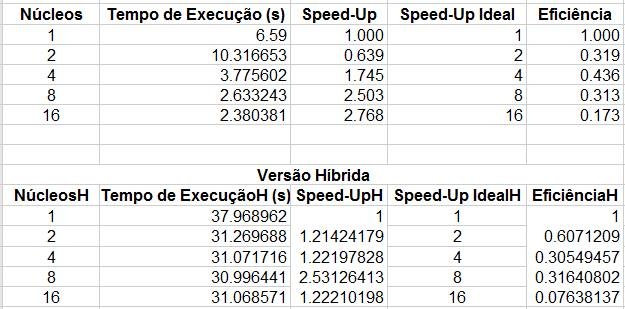
\includegraphics[width=88mm]{table.png}
		\label{fig_graph}
	\end{figure}

	\begin{figure}[H]
		\centering
		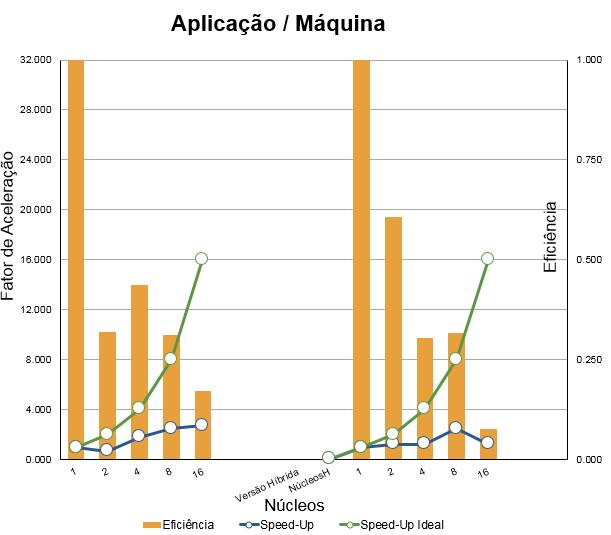
\includegraphics[width=88mm]{graph.png}
		\caption{Gráfico gerado a partir da tabela}
		\label{fig_table}
	\end{figure}

	A diferença entre a troca de mensagens pequenas para mensagens maiores 
	podem ser um dos motivos que impactou no tempo de resposta, já que os processos
	passam a receber mensagens maiores e tem que processalas em paralelo com as 
	threads disponíveis e tira o trabalho do mestre em dividir em trabalhos
	menores para serem realizados. Outra questão é que número de núcleos que os nós 
	possuem, para esse tipo de implementação, pode ser ainda muito baixo para que se 
	obtenha resultados mais satisfatórios. 

	O fato de se estar utilizando quatro nós e a biblioteca MPI junto a OpenMP permite 
	uma menor dependência no mestre e que os pacotes de trabalho a serem ordenados sejam
	realizados pelos nós(($8$ núcleos em cada uma das máquinas com capacidade de simular $16$ 
	threads)) que conseguem explorar um paralilismo com memória compartilhadarealizando
	mais de um pedaço da tarefa ao mesmo tempo para cada processo. Quanto a	distribuição de 
	carga que fica a cargo do MPI o algoritmo consegue distribuir ela igualmente parar 
	os processos que estão ativos nos diferentes nós.

\section{Dificuldades Encontradas}

	Foram encontradas dificuldades quanto ao modo de trabalhar do OpenMP que diminuiram após algumas
	pesquisas de como ele funciona, outras dificuldades encontradas foram relativas ao incremento do tempo
	de execução quando comparado aos do trabalho um e quais são as razoões para esse tempo ter aumentado\@.

\end{document}

